{AOV(Activity On Vertex
network)网{是一种顶点表示活动,边表示活动的先后次序,没有回路的有向图。}}

{对一个有向无环图G进行拓扑排序,是将G中所有顶点排成一个线性序列,使得图中任意一对顶点u和v,若存在从u到v的路径,则u在线性序列中出现在v之前。}

{拓扑排序的步骤为:}

{1. 在有向图中选一个没有前驱的顶点并且输出之。}

{2. 从图中删除该顶点和所有以它为尾的弧。}

{3.
重复上述两步,直至全部顶点均已输出或图中剩余的顶点中都有前驱。后者说明有向图中有环。}

{{\textbf{由于没有前驱的顶点可能不唯一,所以拓扑排序的结果也不唯一,}}如下图所示。}

{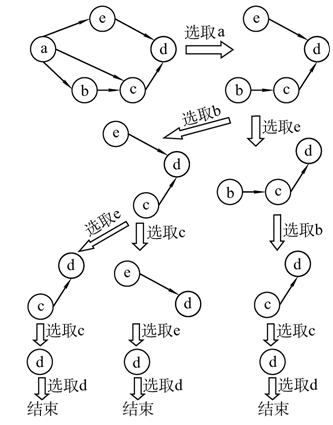
\includegraphics[width=3.70833in,height=4.72917in]{png-jpeg-pics/1BE46EE02D14AF09C8488846718668CB.png}\\
\hspace*{0.333em}}

{故本例有3个不同的拓扑排序序列,分别为:abced、abecd、aebcd。}
